\documentclass{standalone}
\usepackage{tikz}

\definecolor{viridisblue}{RGB}{68,1,84}
\definecolor{viridisyellow}{RGB}{253,231,37}
\definecolor{viridisgreen}{RGB}{35,138,141}

\begin{document}

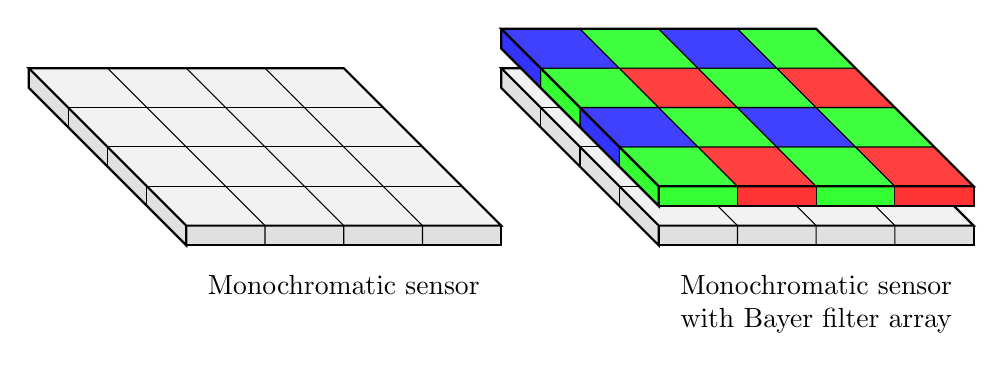
\begin{tikzpicture}[z={(1cm,0cm)},x={(0.5cm,-0.5cm)}, y={(0cm,1cm)}, scale=1]

    % constants
    \def\monol{0}
    \def\monor{4}
    \def\bayerl{6}
    \def\bayerr{10}

    \node [align=center] at (3,0,1.5) {Monochromatic sensor};
    \node [align=center] at (3.5,0,7.25) {\begin{tabular}{c}Monochromatic sensor\\ with Bayer filter array\end{tabular}};
    
    \draw [thick,fill=black!12] (2,0.25,\monol) -- (2,0,\monol) -- (2,0,\monor) -- (2,0.25,\monor);
    \draw [thick,fill=black!12] (2,0.25,\monol) -- (2,0,\monol) -- (-2,0,\monol) -- (-2,0.25,\monol);
    \draw [thick,fill=black!5] (-2,0.25,\monol) -- (-2,0.25,\monor) -- (2,0.25,\monor) -- (2,0.25,\monol) -- cycle; 

    \foreach \z in {1,...,3}
        \draw (2,0,\z) -- (2,0.25,\z) -- (-2,0.25,\z);

    \foreach \x in {-1,...,1}
        \draw (\x,0,\monol) -- (\x,0.25,\monol) -- (\x,0.25,\monor);

    \draw [thick,fill=black!12] (2,0.25,\bayerl) -- (2,0,\bayerl) -- (2,0,\bayerr) -- (2,0.25,\bayerr);
    \draw [thick,fill=black!12] (2,0.25,\bayerl) -- (2,0,\bayerl) -- (-2,0,\bayerl) -- (-2,0.25,\bayerl);
    \draw [thick,fill=black!5] (-2,0.25,\bayerl) -- (-2,0.25,\bayerr) -- (2,0.25,\bayerr) -- (2,0.25,\bayerl) -- cycle; 
    
    \foreach \z in {7,...,9}
        \draw (2,0,\z) -- (2,0.25,\z) -- (-2,0.25,\z);

    \foreach \x in {-1,...,1}
        \draw (\x,0,\bayerl) -- (\x,0.25,\bayerl) -- (\x,0.25,\bayerr);

    % bottom row left to right
    \draw [fill=green!75] (2,0.75,6) -- (2,0.75,7) -- (1,0.75,7) -- (1,0.75,6) -- cycle; % lower left
    \draw [fill=red!75] (2,0.75,7) -- (2,0.75,8) -- (1,0.75,8) -- (1,0.75,7) -- cycle;
    \draw [fill=green!75] (2,0.75,8) -- (2,0.75,9) -- (1,0.75,9) -- (1,0.75,8) -- cycle;
    \draw [fill=red!75] (2,0.75,9) -- (2,0.75,10) -- (1,0.75,10) -- (1,0.75,9) -- cycle;

    \draw [fill=blue!75] (1,0.75,6) -- (1,0.75,7) -- (0,0.75,7) -- (0,0.75,6) -- cycle; % lower left
    \draw [fill=green!75] (1,0.75,7) -- (1,0.75,8) -- (0,0.75,8) -- (0,0.75,7) -- cycle;
    \draw [fill=blue!75] (1,0.75,8) -- (1,0.75,9) -- (0,0.75,9) -- (0,0.75,8) -- cycle;
    \draw [fill=green!75] (1,0.75,9) -- (1,0.75,10) -- (0,0.75,10) -- (0,0.75,9) -- cycle;
    
    \draw [fill=green!75] (0,0.75,6) -- (0,0.75,7) -- (-1,0.75,7) -- (-1,0.75,6) -- cycle; % lower left
    \draw [fill=red!75] (0,0.75,7) -- (0,0.75,8) -- (-1,0.75,8) -- (-1,0.75,7) -- cycle;
    \draw [fill=green!75] (0,0.75,8) -- (0,0.75,9) -- (-1,0.75,9) -- (-1,0.75,8) -- cycle;
    \draw [fill=red!75] (0,0.75,9) -- (0,0.75,10) -- (-1,0.75,10) -- (-1,0.75,9) -- cycle;
    
    \draw [fill=blue!75] (-1,0.75,6) -- (-1,0.75,7) -- (-2,0.75,7) -- (-2,0.75,6) -- cycle; % lower left
    \draw [fill=green!75] (-1,0.75,7) -- (-1,0.75,8) -- (-2,0.75,8) -- (-2,0.75,7) -- cycle;
    \draw [fill=blue!75] (-1,0.75,8) -- (-1,0.75,9) -- (-2,0.75,9) -- (-2,0.75,8) -- cycle;
    \draw [fill=green!75] (-1,0.75,9) -- (-1,0.75,10) -- (-2,0.75,10) -- (-2,0.75,9) -- cycle;
    
    % left edge
    \draw [fill=green!80] (2,0.5,6) -- (2,0.75,6) -- (1,0.75,6) -- (1,0.5,6) --cycle;
    \draw [fill=blue!80] (1,0.5,6) -- (1,0.75,6) -- (0,0.75,6) -- (0,0.5,6) --cycle;
    \draw [fill=green!80] (0,0.5,6) -- (0,0.75,6) -- (-1,0.75,6) -- (-1,0.5,6) --cycle;
    \draw [fill=blue!80] (-1,0.5,6) -- (-1,0.75,6) -- (-2,0.75,6) -- (-2,0.5,6) --cycle;

    %front edge
    \draw [fill=green!80] (2,0.5,6) -- (2,0.75,6) -- (2,0.75,7) -- (2,0.5,7) -- cycle;
    \draw [fill=red!80] (2,0.5,7) -- (2,0.75,7) -- (2,0.75,8) -- (2,0.5,8) -- cycle;
    \draw [fill=green!80] (2,0.5,8) -- (2,0.75,8) -- (2,0.75,9) -- (2,0.5,9) -- cycle;
    \draw [fill=red!80] (2,0.5,9) -- (2,0.75,9) -- (2,0.75,10) -- (2,0.5,10) -- cycle;
   
    \draw [thick] (2,0.75,\bayerl) -- (2,0.5,\bayerl) -- (2,0.5,\bayerr) -- (2,0.75,\bayerr);
    \draw [thick] (2,0.75,\bayerl) -- (2,0.5,\bayerl) -- (-2,0.5,\bayerl) -- (-2,0.75,\bayerl);
    \draw [thick] (-2,0.75,\bayerl) -- (-2,0.75,\bayerr) -- (2,0.75,\bayerr) -- (2,0.75,\bayerl) -- cycle; 

\end{tikzpicture}

\end{document}
